\documentclass[tikz,border=2pt]{standalone}
\usepackage{tikz}
\usetikzlibrary{positioning}
\begin{document}
	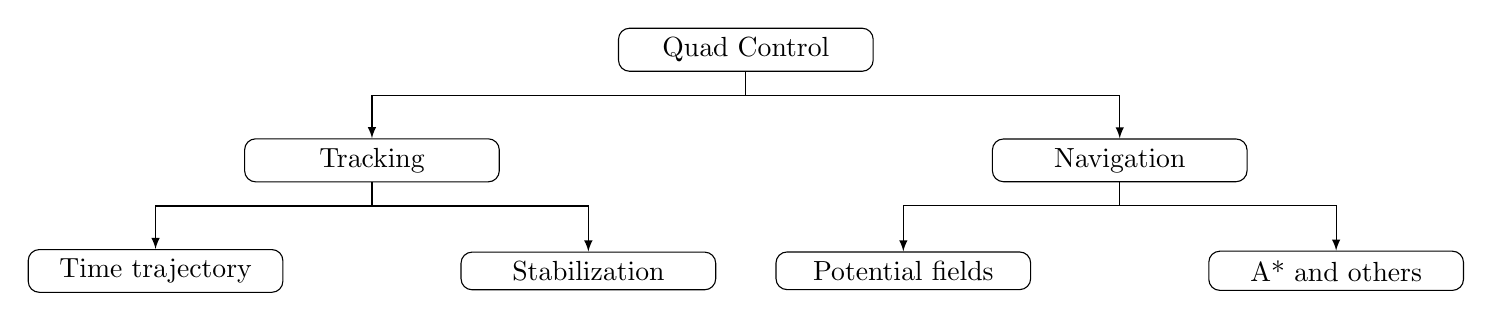
\begin{tikzpicture}[
	main/.style={rectangle, rounded corners, text centered, text width=3cm, draw=black},
	aux/.style={}
	]
				
		\node (control) [main] {Quad Control};
			\node (aux8) [aux, below=of control] {};
			\node (navigation) [main, right=3cm of aux8] {Navigation};
				\node (aux5) [aux, below=of navigation] {};
				\node (potfields) [main, left=of aux5] {Potential fields};
				\node (astar) [main, right=of aux5] {A* and others};
			\node (tracking) [main, left=3cm of aux8] {Tracking};
				\node (aux9) [aux, below=of tracking] {};
				\node (timetraj) [main, left=of aux9] {Time trajectory};
				\node (stabilization) [main, right=of aux9] {Stabilization};
	
	\draw [-latex] (control.south)--++(0,-.3)-| (navigation.north);
	\draw [-latex] (control.south)--++(0,-.3)-| (tracking.north);
	
	\draw [-latex] (tracking.south)--++(0,-.3)-| (timetraj.north);
	\draw [-latex] (tracking.south)--++(0,-.3)-| (stabilization.north);
	
	\draw [-latex] (navigation.south)--++(0,-.3)-| (potfields.north);
	\draw [-latex] (navigation.south)--++(0,-.3)-| (astar.north);
	
	
	\end{tikzpicture}
\end{document}